% This article has been prepared for publication in Energy Economics in RStudio with knitr.
% According to http://www.elsevier.com/author-schemas/the-elsarticle-latex-document-class, we should be using the
% elsarticle.cls file.
% According to http://cdn.elsevier.com/assets/pdf_file/0006/109392/journal_refstyles.pdf, we should be using
% elsarticle-template-2-harv.tex as the template for the text.
% Furthermore, we should be using model2-names.bst for the bibliographic references.
% The approach here is to load the frontmatter and backmatter from elsarticle-template-2-harv.tex
% both ahead of and behind the text for our paper.
% -- Matthew Kuperus Heun, 2013-01-18

%% This is file `elsarticle-template-2-harv.tex',
%%
%% Copyright 2009 Elsevier Ltd
%%
%% This file is part of the 'Elsarticle  Bundle'.
%% ---------------------------------------------
%%
%% It may be distributed under the conditions of the LaTeX Project Public
%% License, either version 1.2 of this license or (at your option) any
%% later version.  The latest version of this license is in
%%    http://www.latex-project.org/lppl.txt
%% and version 1.2 or later is part of all distributions of LaTeX
%% version 1999/12/01 or later.
%%
%% The list of all files belonging to the 'Elsarticle Bundle' is
%% given in the file `manifest.txt'.
%%
%% Template article for Elsevier's document class `elsarticle'
%% with harvard style bibliographic references
%%
%% $Id: elsarticle-template-2-harv.tex 155 2009-10-08 05:35:05Z rishi $
%% $URL: http://lenova.river-valley.com/svn/elsbst/trunk/elsarticle-template-2-harv.tex $
%%
\documentclass[preprint,authoryear,12pt]{elsarticle}\usepackage{graphicx, color}
%% maxwidth is the original width if it is less than linewidth
%% otherwise use linewidth (to make sure the graphics do not exceed the margin)
\makeatletter
\def\maxwidth{ %
  \ifdim\Gin@nat@width>\linewidth
    \linewidth
  \else
    \Gin@nat@width
  \fi
}
\makeatother

\IfFileExists{upquote.sty}{\usepackage{upquote}}{}
\definecolor{fgcolor}{rgb}{0.2, 0.2, 0.2}
\newcommand{\hlnumber}[1]{\textcolor[rgb]{0,0,0}{#1}}%
\newcommand{\hlfunctioncall}[1]{\textcolor[rgb]{0.501960784313725,0,0.329411764705882}{\textbf{#1}}}%
\newcommand{\hlstring}[1]{\textcolor[rgb]{0.6,0.6,1}{#1}}%
\newcommand{\hlkeyword}[1]{\textcolor[rgb]{0,0,0}{\textbf{#1}}}%
\newcommand{\hlargument}[1]{\textcolor[rgb]{0.690196078431373,0.250980392156863,0.0196078431372549}{#1}}%
\newcommand{\hlcomment}[1]{\textcolor[rgb]{0.180392156862745,0.6,0.341176470588235}{#1}}%
\newcommand{\hlroxygencomment}[1]{\textcolor[rgb]{0.43921568627451,0.47843137254902,0.701960784313725}{#1}}%
\newcommand{\hlformalargs}[1]{\textcolor[rgb]{0.690196078431373,0.250980392156863,0.0196078431372549}{#1}}%
\newcommand{\hleqformalargs}[1]{\textcolor[rgb]{0.690196078431373,0.250980392156863,0.0196078431372549}{#1}}%
\newcommand{\hlassignement}[1]{\textcolor[rgb]{0,0,0}{\textbf{#1}}}%
\newcommand{\hlpackage}[1]{\textcolor[rgb]{0.588235294117647,0.709803921568627,0.145098039215686}{#1}}%
\newcommand{\hlslot}[1]{\textit{#1}}%
\newcommand{\hlsymbol}[1]{\textcolor[rgb]{0,0,0}{#1}}%
\newcommand{\hlprompt}[1]{\textcolor[rgb]{0.2,0.2,0.2}{#1}}%

\usepackage{framed}
\makeatletter
\newenvironment{kframe}{%
 \def\at@end@of@kframe{}%
 \ifinner\ifhmode%
  \def\at@end@of@kframe{\end{minipage}}%
  \begin{minipage}{\columnwidth}%
 \fi\fi%
 \def\FrameCommand##1{\hskip\@totalleftmargin \hskip-\fboxsep
 \colorbox{shadecolor}{##1}\hskip-\fboxsep
     % There is no \\@totalrightmargin, so:
     \hskip-\linewidth \hskip-\@totalleftmargin \hskip\columnwidth}%
 \MakeFramed {\advance\hsize-\width
   \@totalleftmargin\z@ \linewidth\hsize
   \@setminipage}}%
 {\par\unskip\endMakeFramed%
 \at@end@of@kframe}
\makeatother

\definecolor{shadecolor}{rgb}{.97, .97, .97}
\definecolor{messagecolor}{rgb}{0, 0, 0}
\definecolor{warningcolor}{rgb}{1, 0, 1}
\definecolor{errorcolor}{rgb}{1, 0, 0}
\newenvironment{knitrout}{}{} % an empty environment to be redefined in TeX

\usepackage{alltt}

%% Use the option review to obtain double line spacing
%% \documentclass[authoryear,preprint,review,12pt]{elsarticle}

%% Use the options 1p,twocolumn; 3p; 3p,twocolumn; 5p; or 5p,twocolumn
%% for a journal layout:
%% \documentclass[final,authoryear,1p,times]{elsarticle}
%% \documentclass[final,authoryear,1p,times,twocolumn]{elsarticle}
%% \documentclass[final,authoryear,3p,times]{elsarticle}
%% \documentclass[final,authoryear,3p,times,twocolumn]{elsarticle}
%% \documentclass[final,authoryear,5p,times]{elsarticle}
%% \documentclass[final,authoryear,5p,times,twocolumn]{elsarticle}

%% if you use PostScript figures in your article
%% use the graphics package for simple commands
%% \usepackage{graphics}
%% or use the graphicx package for more complicated commands
%% \usepackage{graphicx}
%% or use the epsfig package if you prefer to use the old commands
%% \usepackage{epsfig}

%% The amssymb package provides various useful mathematical symbols
\usepackage{amssymb}
%% The amsthm package provides extended theorem environments
%% \usepackage{amsthm}

\usepackage{soul} %Provides strikethrough text
\usepackage{float} %Allows precise positioning of tables and figures within the text

%% The lineno packages adds line numbers. Start line numbering with
%% \begin{linenumbers}, end it with \end{linenumbers}. Or switch it on
%% for the whole article with \linenumbers after \end{frontmatter}.
%% \usepackage{lineno}

%% natbib.sty is loaded by default. However, natbib options can be
%% provided with \biboptions{...} command. Following options are
%% valid:

%%   round  -  round parentheses are used (default)
%%   square -  square brackets are used   [option]
%%   curly  -  curly braces are used      {option}
%%   angle  -  angle brackets are used    <option>
%%   semicolon  -  multiple citations separated by semi-colon (default)
%%   colon  - same as semicolon, an earlier confusion
%%   comma  -  separated by comma
%%   authoryear - selects author-year citations (default)
%%   numbers-  selects numerical citations
%%   super  -  numerical citations as superscripts
%%   sort   -  sorts multiple citations according to order in ref. list
%%   sort&compress   -  like sort, but also compresses numerical citations
%%   compress - compresses without sorting
%%   longnamesfirst  -  makes first citation full author list
%%
%% \biboptions{longnamesfirst,comma}

% \biboptions{}

\journal{Energy Economics}

\begin{document}

\begin{frontmatter}

%% Title, authors and addresses

%% use the tnoteref command within \title for footnotes;
%% use the tnotetext command for the associated footnote;
%% use the fnref command within \author or \address for footnotes;
%% use the fntext command for the associated footnote;
%% use the corref command within \author for corresponding author footnotes;
%% use the cortext command for the associated footnote;
%% use the ead command for the email address,
%% and the form \ead[url] for the home page:
%%
%% \title{Title\tnoteref{label1}}
%% \tnotetext[label1]{}
%% \author{Name\corref{cor1}\fnref{label2}}
%% \ead{email address}
%% \ead[url]{home page}
%% \fntext[label2]{}
%% \cortext[cor1]{}
%% \address{Address\fnref{label3}}
%% \fntext[label3]{}

\title{An Empirical Analysis of the Role of Energy in Economic Growth}

%% use optional labels to link authors explicitly to addresses:
%% \author[label1,label2]{<author name>}
%% \address[label1]{<address>}
%% \address[label2]{<address>}

\author[Calvin]{Caleb Reese}
\author[Calvin]{Lucas Timmer}
\author[Stellenbosch]{Martin de Wit}
\author[Calvin]{Matthew Kuperus Heun\corref{cor1}}
\ead{mkh2@calvin.edu, tel: +1 (616) 526-6663, fax: +1 (616) 526-6501}

\cortext[cor1]{Corresponding author}
\address[Calvin]{Engineering Department, Calvin College, Grand Rapids, MI 49546, USA}
\address[Stellenbosch]{ Stellenbosch University, School of Public Leadership, P.O. Box 610, Bellville 7535, South Africa}

\begin{abstract}
%% Text of abstract
*********** Add abstract ***********
\end{abstract}

\begin{keyword}
%% keywords here, in the form: keyword \sep keyword
economic growth \sep energy \sep cobb-douglas \sep CES \sep LINEX
%% MSC codes here, in the form: \MSC code \sep code
%% or \MSC[2008] code \sep code (2000 is the default)
\end{keyword}

\end{frontmatter}

% \linenumbers
%% main text

\section*{To-do List}
\begin{itemize}
\item Reese: Add text from Word verson of paper to the LaTeX version.
\item Heun: Add setup variables for figure height and width where not already included.
\item Heun: Deal with missing covariance numbers when columns have unequal length.
\item Heun: Add single factor fits
      \begin{itemize}
      \item \st{GDP comparison graph}
      \item parameter graphs ($\lambda$ and $m$) for each country
      \item parameter tables for each country in the appendix
      \item \st{AIC rows in the AIC table}
      \end{itemize}
\item Heun: Add CES production function fits
      \begin{itemize}
      \item GDP comparison graph
      \item parameter graphs ($\lambda$ and $m$) for each country
      \item parameter tables for each country in the appendix
      \item AIC rows in the AIC table
      \end{itemize}
\item Heun: Add Linex production function fits
      \begin{itemize}
      \item GDP comparison graph
      \item parameter graphs ($\lambda$ and $m$) for each country
      \item parameter tables for each country in the appendix
      \item AIC rows in the AIC table
      \end{itemize}
\item Heun: Eliminate blanks in the coefficient tables for the 95\% CIs in the Cobb-Douglas with energy rows. Asked Pruim about this via email but have not heard a response.
      \begin{itemize}
      \item ZA: lower bound on $\lambda$ and upper bound on $\alpha$
      \item ZM: lower bound on $\lambda$
      \end{itemize}
\item Heun: Fix warnings of the form ``Warning:  step factor 0.000488281 reduced below ’minFactor’ of 0.000976562'' in the code that generates the Cobb-Douglas with energy fits.
\item \st{Heun: Create a table of AIC values for each fit.}
\item \st{Heun: Add $u$ predictions for Cobb-Douglas}
\item \st{Heun: move tables to an appendix at the end.}
\item \st{Heun: Add acknowledgements (Dad, Pruim)}
\item \st{Heun: Add $u$ parameter table and graph}
\item \st{Heun: Add covariance metrics.}
\end{itemize}

%%%%%%%%%%%%%%%%%%%%%%%%%%%%%%%
\section{Introduction}
%%%%%%%%%%%%%%%%%%%%%%%%%%%%%%%

*********** Caleb, put your LaTeX code here. *************









%%%%%%%%%%%%%%%%%%%%%%%%%%%%%%%
\section{Historical Data}
%%%%%%%%%%%%%%%%%%%%%%%%%%%%%%%

Figure \ref{fig:Factors_Lattice_Graph} shows historical data, including GDP ($y$), capital stock ($k$), labor ($l$), and the various energy types ($q$, $x$, and $u$). Facotrs of production track each other closely, and large covariances among these variables can be seen in Tables \ref{tab:Covariance_US} through \ref{tab:Covariance_ZM}.

\begin{knitrout}
\definecolor{shadecolor}{rgb}{0.969, 0.969, 0.969}\color{fgcolor}\begin{figure}[H]

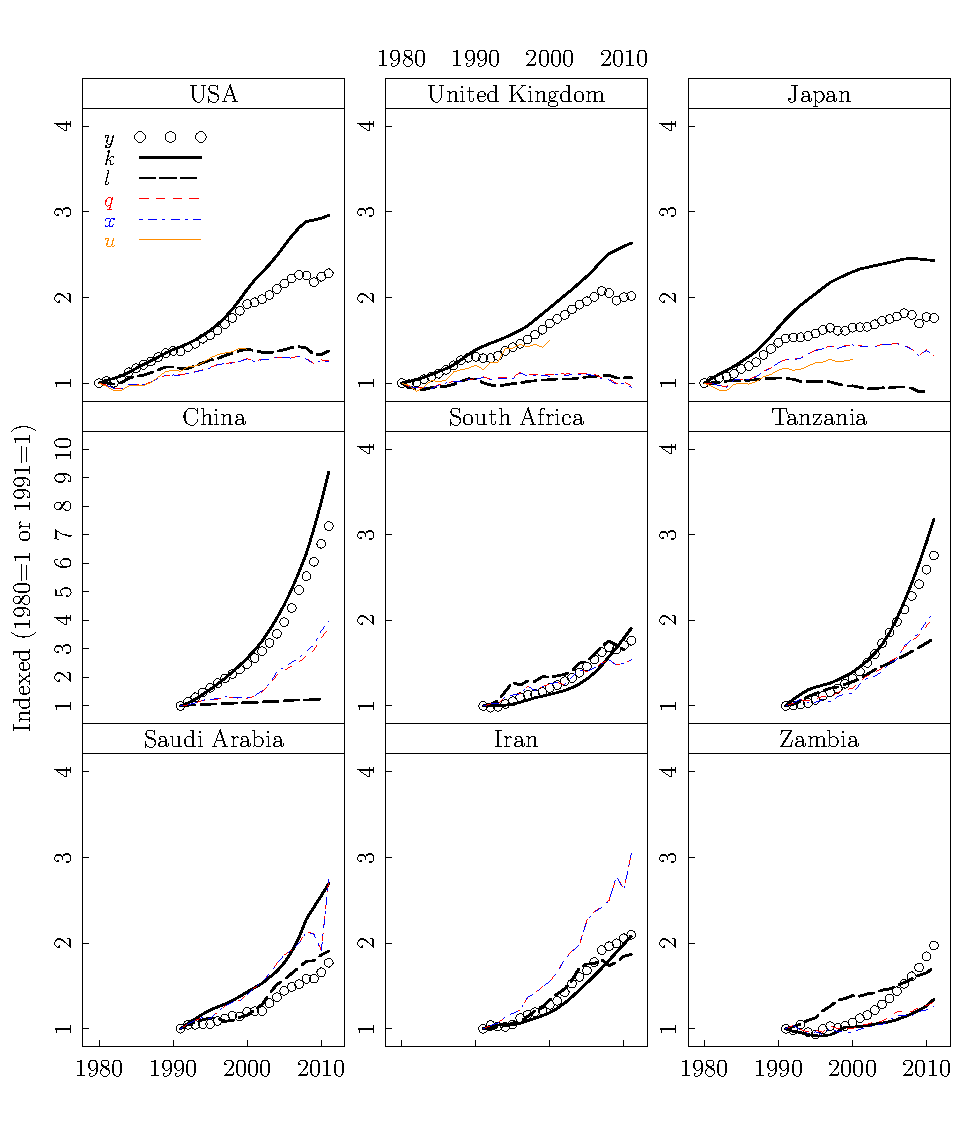
\includegraphics[width=\maxwidth]{figure/Factors_Lattice_Graph} \caption[Historical data]{Historical data. Indexed GDP ($y$), capital stock ($k$), labor ($l$), thermal energy ($q$), exergy ($x$), and useful work ($u$).\label{fig:Factors_Lattice_Graph}}
\end{figure}


\end{knitrout}


%%%%%%%%%%%%%%%%%%%%%%%%%%%%%%%
\section{Single-factor Models (SF)}
%%%%%%%%%%%%%%%%%%%%%%%%%%%%%%%




We begin by fitting single-factor economic models of the form

\begin{equation} \label{eq:Single_Factor_Generic}
  y = a^{\lambda (t-t_0)}f^{m}
\end{equation}

\noindent to historical data where the factor of production ($f$) is any of $k$, $l$, $q$, $x$, or $u$, and the exponent ($m$) is $\alpha$ for $k$, $\beta$ for $l$, or $\gamma$ for $q$, $x$, or $u$.

Figure \ref{fig:SF_GDP_Lattice_Graph} compares single-factor model predictions with historica data.

\begin{knitrout}
\definecolor{shadecolor}{rgb}{0.969, 0.969, 0.969}\color{fgcolor}\begin{figure}[H]

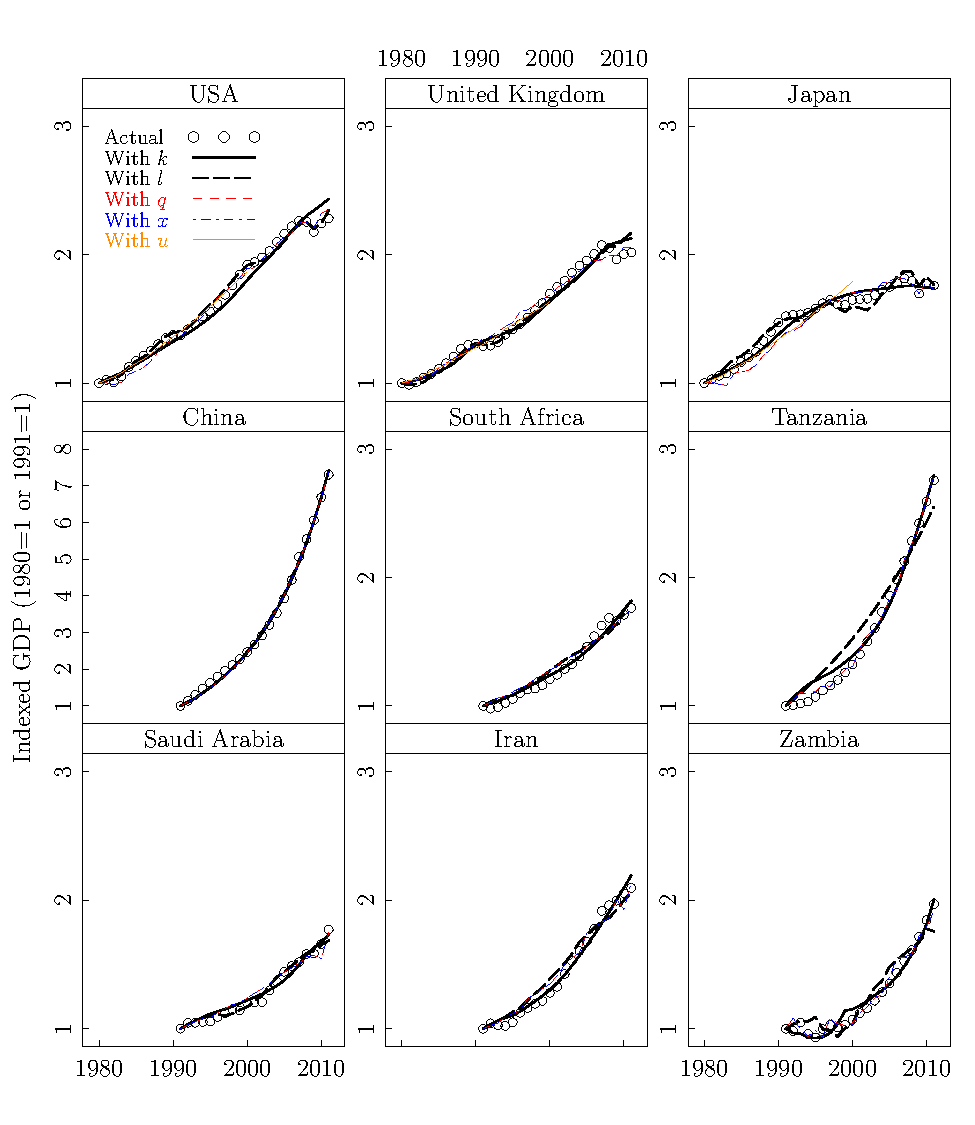
\includegraphics[width=\maxwidth]{figure/SF_GDP_Lattice_Graph} \caption[Single-factor results]{Single-factor results.\label{fig:SF_GDP_Lattice_Graph}}
\end{figure}


\end{knitrout}


%%%%%%%%%%%%%%%%%%%%%%%%%%%%%%%
\section{Cobb-Douglas Models Without Energy (CD)}
%%%%%%%%%%%%%%%%%%%%%%%%%%%%%%%




The Cobb-Douglas model without energy is given by

\begin{equation} \label{eq:CD_No_Energy}
  y = a^{\lambda (t-t_0)}k^{\alpha}l^{\beta}.
\end{equation}

Figure \ref{fig:CD_Params_Graph} shows values and 95\% confidence intervals for the parameters for the Cobb-Douglas model (without energy).

\begin{knitrout}
\definecolor{shadecolor}{rgb}{0.969, 0.969, 0.969}\color{fgcolor}\begin{figure}[H]

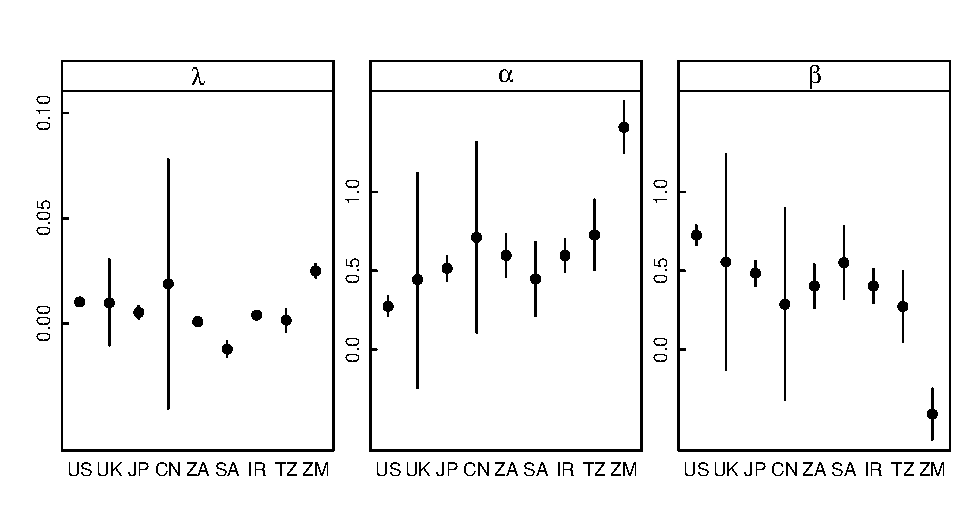
\includegraphics[width=\maxwidth]{figure/CD_Params_Graph} \caption[Cobb-Douglas (without energy) model parameters]{Cobb-Douglas (without energy) model parameters. Vertical bars indicate 95\% confidence intervals.\label{fig:CD_Params_Graph}}
\end{figure}


\end{knitrout}


\section{Cobb-Douglas Models With Energy (CDe)}

We can force $\alpha$, $\beta$, and $\gamma$ to be in $[0,1]$ by a reparameterization:

$a \in[0,1], b \in [0,1], \alpha=\min(a,b), \beta=|b-a|, \gamma = 1-\max(a,b)$

The Cobb-Douglas model with energy is given by

\begin{equation} \label{eq:CD_With_Energy}
  y = a^{\lambda (t-t_0)}k^{\alpha}l^{\beta}e^{\gamma},
\end{equation}

\noindent where $e$ can be any of thermal energy ($q$), exergy ($x$), or useful work ($u$).

\subsection{Cobb-Douglas with thermal energy ($q$)}

Figure \ref{fig:CDq_Params_Graph} shows values and 95\% confidence intervals for the parameters for the Cobb-Douglas model (with $q$).

\begin{knitrout}
\definecolor{shadecolor}{rgb}{0.969, 0.969, 0.969}\color{fgcolor}\begin{figure}[H]

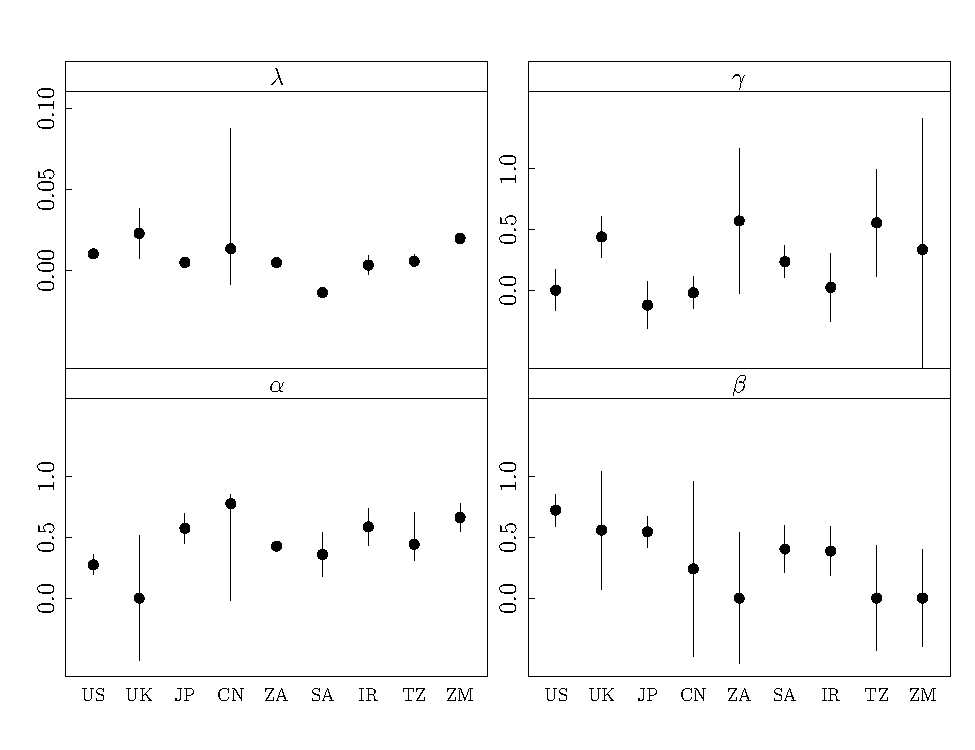
\includegraphics[width=\maxwidth]{figure/CDq_Params_Graph} \caption[Cobb-Douglas (with $q$) model parameters]{Cobb-Douglas (with $q$) model parameters. Vertical bars indicate 95\% confidence intervals.\label{fig:CDq_Params_Graph}}
\end{figure}


\end{knitrout}


\subsection{Cobb-Douglas with exergy ($x$)}

The Cobb-Douglas (with exergy) parameters are given in Table \ref{tab:CD_Parameters_With_X}.

Figure \ref{fig:CDx_Params_Graph} shows values and 95\% confidence intervals for the parameters for the Cobb-Douglas model (with $x$).

\begin{knitrout}
\definecolor{shadecolor}{rgb}{0.969, 0.969, 0.969}\color{fgcolor}\begin{figure}[H]

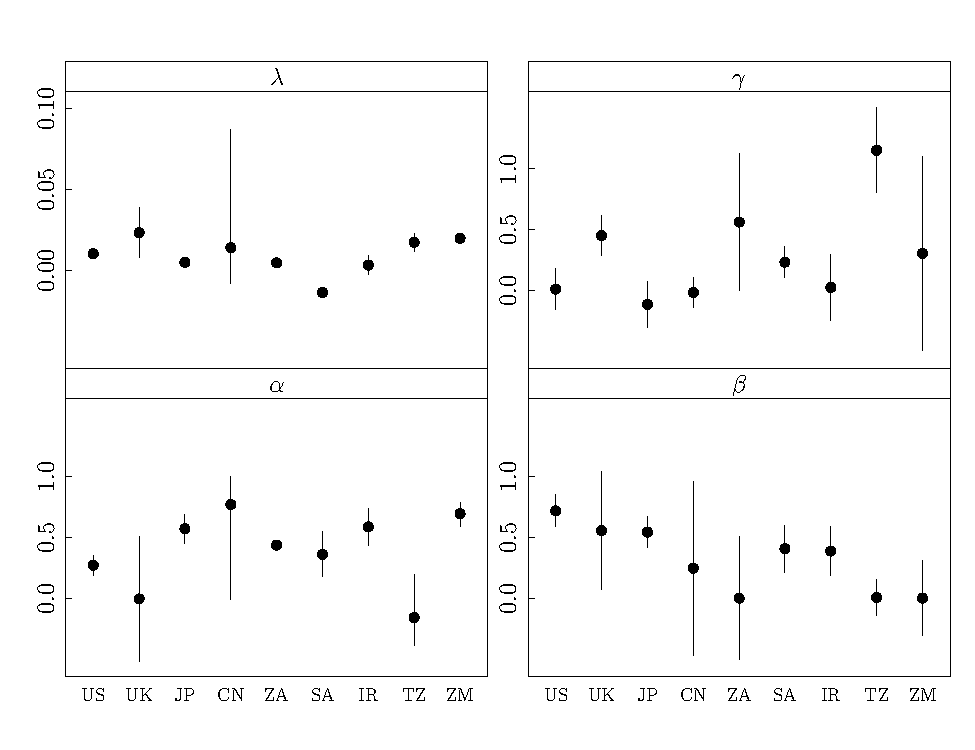
\includegraphics[width=\maxwidth]{figure/CDx_Params_Graph} \caption[Cobb-Douglas (with $x$) model parameters]{Cobb-Douglas (with $x$) model parameters. Vertical bars indicate 95\% confidence intervals.\label{fig:CDx_Params_Graph}}
\end{figure}


\end{knitrout}


\subsection{Cobb-Douglas with useful work ($u$)}

Figure \ref{fig:CDu_Params_Graph} shows values and 95\% confidence intervals for the parameters for the Cobb-Douglas model (with $u$).

\begin{knitrout}
\definecolor{shadecolor}{rgb}{0.969, 0.969, 0.969}\color{fgcolor}\begin{figure}[H]

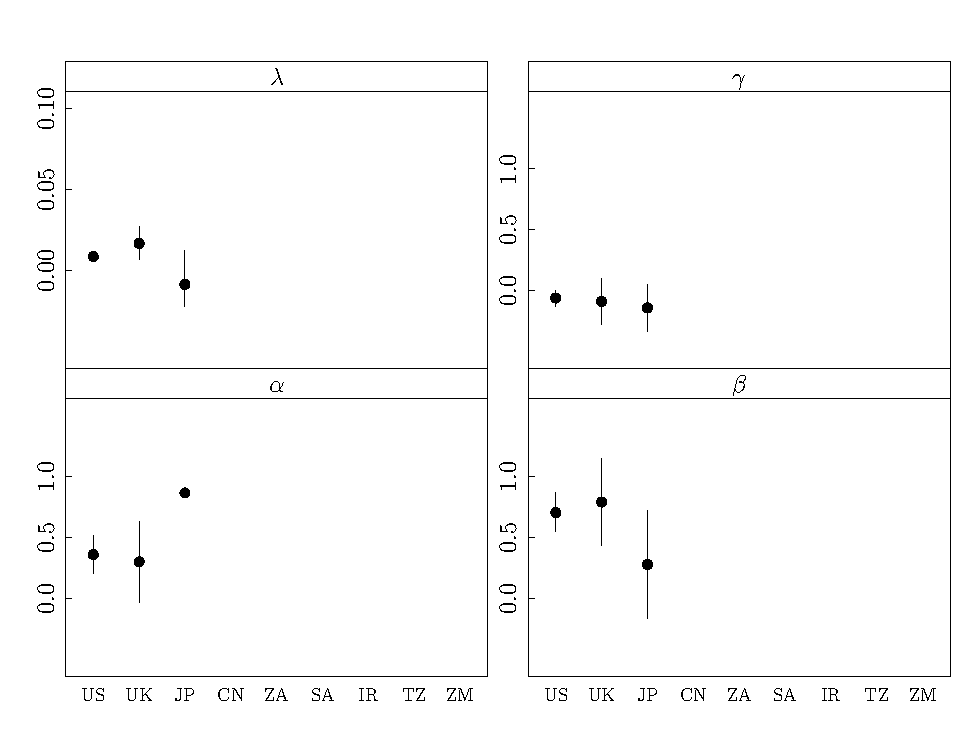
\includegraphics[width=\maxwidth]{figure/CDu_Params_Graph} \caption[Cobb-Douglas (with $u$) model parameters]{Cobb-Douglas (with $u$) model parameters. Vertical bars indicate 95\% confidence intervals.\label{fig:CDu_Params_Graph}}
\end{figure}


\end{knitrout}


\subsection{Cobb-Douglas Comparisons}

Figure \ref{fig:CD_GDP_Lattice_Graph} compares predictions from the Cobb-Douglas models (without energy, with $Q$, and with $x$) to historical data.

\begin{knitrout}
\definecolor{shadecolor}{rgb}{0.969, 0.969, 0.969}\color{fgcolor}\begin{figure}[H]

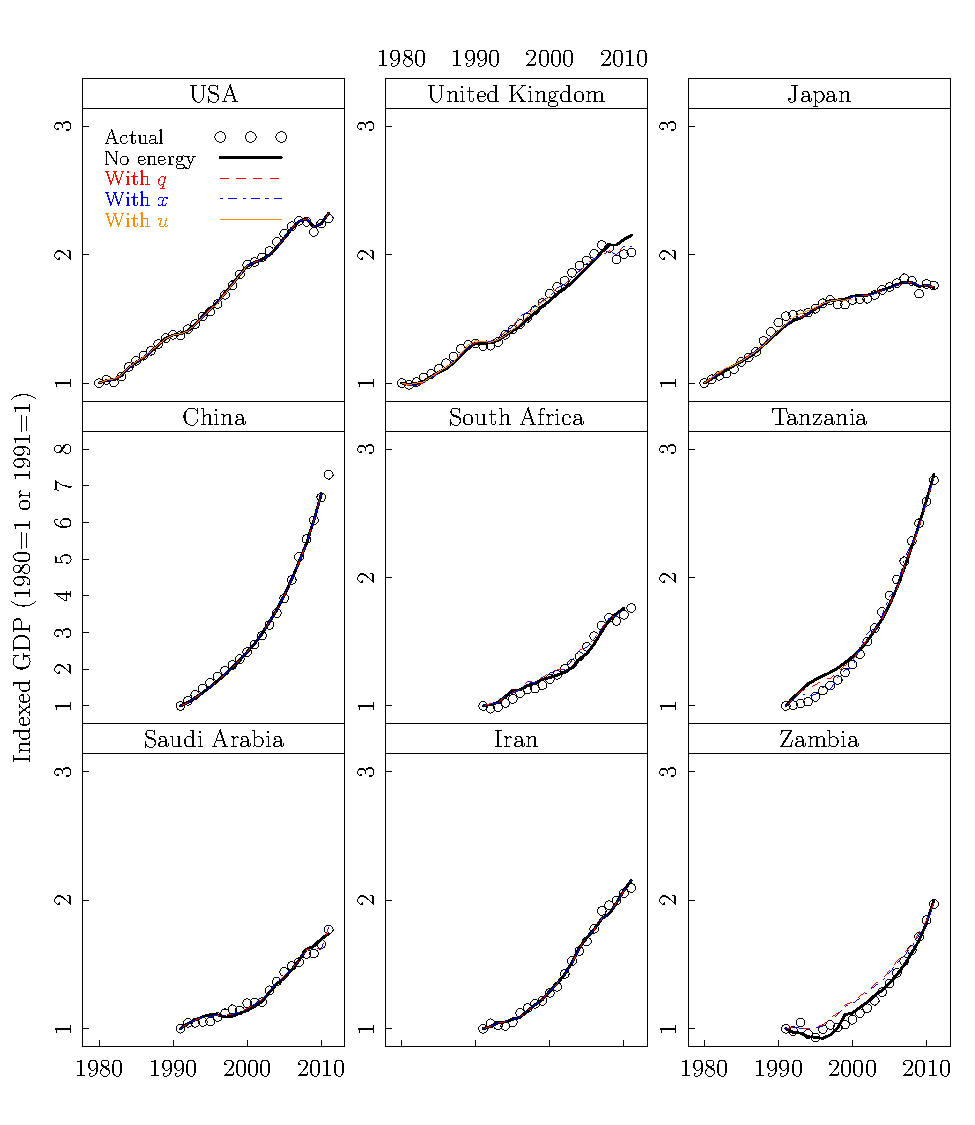
\includegraphics[width=\maxwidth]{figure/CD_GDP_Lattice_Graph} \caption[Cobb-Douglas results]{Cobb-Douglas results.\label{fig:CD_GDP_Lattice_Graph}}
\end{figure}


\end{knitrout}


%%%%%%%%%%%%%%%%%%%%%%%%%%%%%%%
\section{CES Models}
%%%%%%%%%%%%%%%%%%%%%%%%%%%%%%%




\subsection{CES with $Q$}







\subsection{CES with $X$}

\subsection{CES with $U$}

%%%%%%%%%%%%%%%%%%%%%%%%%%%%%%%
\section{LINEX Models}
%%%%%%%%%%%%%%%%%%%%%%%%%%%%%%%

\subsection{LINEX with $Q$}

\subsection{LINEX with $X$}

\subsection{LINEX with $U$}

%%%%%%%%%%%%%%%%%%%%%%%%%%%%%%%
\section{Conclusion}
%%%%%%%%%%%%%%%%%%%%%%%%%%%%%%%

****************** Add conclusion here. *********************

%%%%%%%%%%%%%%%%%%%%%%%%%%%%%%%
\section*{Acknowledgements}
%%%%%%%%%%%%%%%%%%%%%%%%%%%%%%%

Funding for Caleb Reese and Lucas Timmer was graciously supplied by the Jack and Lois Kuipers Applied Mathematics Endowment and the Calvin College Alumni Association. The authors thank Randall Pruim (Calvin College) and Loren L. Heun (Western Michigan University) for their insightful comments on and invaluable assistance with the statistical analyses presented herein.

%% The Appendices part is started with the command \appendix;
%% appendix sections are then done as normal sections
%% \appendix
%% \section{}
%% \label{}

%%%%%%%%%%%%%%%%%%%%%%%%%%%%%%%
\appendix
%%%%%%%%%%%%%%%%%%%%%%%%%%%%%%%

%%%%%%%%%%%%%%%%%%%%%%%%%%%%%%%
\section{Covariance Tables}
\setcounter{table}{0} % Restarts table number counter at 0 in this section.
%%%%%%%%%%%%%%%%%%%%%%%%%%%%%%%

The following tables show covariances among GDP ($y$) and factors of production ($k$, $l$, $q$, $x$, and $u$).

% latex table generated in R 2.15.2 by xtable 1.7-0 package
% Sun Feb 10 22:10:42 2013
\begin{table}[H]
\begin{center}
\caption{Covariance table for  US economy.}
\label{tab:Covariance_US}
\begin{tabular}{rrrrrrr}
  \hline
 & $y$ & $k$ & $l$ & $q$ & $x$ & $u$ \\ 
  \hline
$y$ & 1.00 & 0.99 & 0.95 & 0.95 & 0.95 &  \\ 
  $k$ & 0.99 & 1.00 & 0.88 & 0.89 & 0.88 &  \\ 
  $l$ & 0.95 & 0.88 & 1.00 & 0.98 & 0.98 &  \\ 
  $q$ & 0.95 & 0.89 & 0.98 & 1.00 & 1.00 &  \\ 
  $x$ & 0.95 & 0.88 & 0.98 & 1.00 & 1.00 &  \\ 
  $u$ &  &  &  &  &  & 1.00 \\ 
   \hline
\end{tabular}
\end{center}
\end{table}



% latex table generated in R 2.15.2 by xtable 1.7-0 package
% Sun Feb 10 22:10:42 2013
\begin{table}[H]
\begin{center}
\caption{Covariance table for  UK economy.}
\label{tab:Covariance_UK}
\begin{tabular}{rrrrrrr}
  \hline
 & $y$ & $k$ & $l$ & $q$ & $x$ & $u$ \\ 
  \hline
$y$ & 1.00 & 0.99 & 0.89 & 0.53 & 0.47 &  \\ 
  $k$ & 0.99 & 1.00 & 0.85 & 0.43 & 0.36 &  \\ 
  $l$ & 0.89 & 0.85 & 1.00 & 0.56 & 0.52 &  \\ 
  $q$ & 0.53 & 0.43 & 0.56 & 1.00 & 1.00 &  \\ 
  $x$ & 0.47 & 0.36 & 0.52 & 1.00 & 1.00 &  \\ 
  $u$ &  &  &  &  &  & 1.00 \\ 
   \hline
\end{tabular}
\end{center}
\end{table}



% latex table generated in R 2.15.2 by xtable 1.7-0 package
% Sun Feb 10 22:10:42 2013
\begin{table}[H]
\begin{center}
\caption{Covariance table for  JP economy.}
\label{tab:Covariance_JP}
\begin{tabular}{rrrrrrr}
  \hline
 & $y$ & $k$ & $l$ & $q$ & $x$ & $u$ \\ 
  \hline
$y$ & 1.00 & 0.98 & -0.62 & 0.96 & 0.96 &  \\ 
  $k$ & 0.98 & 1.00 & -0.72 & 0.96 & 0.96 &  \\ 
  $l$ & -0.62 & -0.72 & 1.00 & -0.55 & -0.55 &  \\ 
  $q$ & 0.96 & 0.96 & -0.55 & 1.00 & 1.00 &  \\ 
  $x$ & 0.96 & 0.96 & -0.55 & 1.00 & 1.00 &  \\ 
  $u$ &  &  &  &  &  & 1.00 \\ 
   \hline
\end{tabular}
\end{center}
\end{table}



% latex table generated in R 2.15.2 by xtable 1.7-0 package
% Sun Feb 10 22:10:42 2013
\begin{table}[H]
\begin{center}
\caption{Covariance table for  CN economy.}
\label{tab:Covariance_CN}
\begin{tabular}{rrrrrr}
  \hline
 & $y$ & $k$ & $l$ & $q$ & $x$ \\ 
  \hline
$y$ & 1.00 & 1.00 &  & 0.99 & 0.99 \\ 
  $k$ & 1.00 & 1.00 &  & 0.99 & 0.99 \\ 
  $l$ &  &  & 1.00 &  &  \\ 
  $q$ & 0.99 & 0.99 &  & 1.00 & 1.00 \\ 
  $x$ & 0.99 & 0.99 &  & 1.00 & 1.00 \\ 
   \hline
\end{tabular}
\end{center}
\end{table}



% latex table generated in R 2.15.2 by xtable 1.7-0 package
% Sun Feb 10 22:10:42 2013
\begin{table}[H]
\begin{center}
\caption{Covariance table for  ZA economy.}
\label{tab:Covariance_ZA}
\begin{tabular}{rrrrrr}
  \hline
 & $y$ & $k$ & $l$ & $q$ & $x$ \\ 
  \hline
$y$ & 1.00 & 0.96 &  & 0.97 & 0.97 \\ 
  $k$ & 0.96 & 1.00 &  & 0.89 & 0.89 \\ 
  $l$ &  &  & 1.00 &  &  \\ 
  $q$ & 0.97 & 0.89 &  & 1.00 & 1.00 \\ 
  $x$ & 0.97 & 0.89 &  & 1.00 & 1.00 \\ 
   \hline
\end{tabular}
\end{center}
\end{table}



% latex table generated in R 2.15.2 by xtable 1.7-0 package
% Sun Feb 10 22:10:42 2013
\begin{table}[H]
\begin{center}
\caption{Covariance table for  SA economy.}
\label{tab:Covariance_SA}
\begin{tabular}{rrrrrr}
  \hline
 & $y$ & $k$ & $l$ & $q$ & $x$ \\ 
  \hline
$y$ & 1.00 & 0.99 & 0.99 & 0.97 & 0.97 \\ 
  $k$ & 0.99 & 1.00 & 0.97 & 0.95 & 0.95 \\ 
  $l$ & 0.99 & 0.97 & 1.00 & 0.95 & 0.95 \\ 
  $q$ & 0.97 & 0.95 & 0.95 & 1.00 & 1.00 \\ 
  $x$ & 0.97 & 0.95 & 0.95 & 1.00 & 1.00 \\ 
   \hline
\end{tabular}
\end{center}
\end{table}



% latex table generated in R 2.15.2 by xtable 1.7-0 package
% Sun Feb 10 22:10:42 2013
\begin{table}[H]
\begin{center}
\caption{Covariance table for  IR economy.}
\label{tab:Covariance_IR}
\begin{tabular}{rrrrrr}
  \hline
 & $y$ & $k$ & $l$ & $q$ & $x$ \\ 
  \hline
$y$ & 1.00 & 0.99 & 0.97 & 0.99 & 0.99 \\ 
  $k$ & 0.99 & 1.00 & 0.93 & 0.98 & 0.98 \\ 
  $l$ & 0.97 & 0.93 & 1.00 & 0.97 & 0.97 \\ 
  $q$ & 0.99 & 0.98 & 0.97 & 1.00 & 1.00 \\ 
  $x$ & 0.99 & 0.98 & 0.97 & 1.00 & 1.00 \\ 
   \hline
\end{tabular}
\end{center}
\end{table}



% latex table generated in R 2.15.2 by xtable 1.7-0 package
% Sun Feb 10 22:10:42 2013
\begin{table}[H]
\begin{center}
\caption{Covariance table for  TZ economy.}
\label{tab:Covariance_TZ}
\begin{tabular}{rrrrrr}
  \hline
 & $y$ & $k$ & $l$ & $q$ & $x$ \\ 
  \hline
$y$ & 1.00 & 0.99 & 0.98 & 1.00 & 1.00 \\ 
  $k$ & 0.99 & 1.00 & 0.96 & 0.99 & 0.99 \\ 
  $l$ & 0.98 & 0.96 & 1.00 & 0.98 & 0.97 \\ 
  $q$ & 1.00 & 0.99 & 0.98 & 1.00 & 1.00 \\ 
  $x$ & 1.00 & 0.99 & 0.97 & 1.00 & 1.00 \\ 
   \hline
\end{tabular}
\end{center}
\end{table}



% latex table generated in R 2.15.2 by xtable 1.7-0 package
% Sun Feb 10 22:10:42 2013
\begin{table}[H]
\begin{center}
\caption{Covariance table for  ZM economy.}
\label{tab:Covariance_ZM}
\begin{tabular}{rrrrrr}
  \hline
 & $y$ & $k$ & $l$ & $q$ & $x$ \\ 
  \hline
$y$ & 1.00 & 0.98 & 0.88 & 0.98 & 0.96 \\ 
  $k$ & 0.98 & 1.00 & 0.87 & 0.96 & 0.94 \\ 
  $l$ & 0.88 & 0.87 & 1.00 & 0.86 & 0.79 \\ 
  $q$ & 0.98 & 0.96 & 0.86 & 1.00 & 0.99 \\ 
  $x$ & 0.96 & 0.94 & 0.79 & 0.99 & 1.00 \\ 
   \hline
\end{tabular}
\end{center}
\end{table}



%%%%%%%%%%%%%%%%%%%%%%%%%%%%%%%
\section{Model Parameters}
\setcounter{table}{0} % Restarts table number counter at 0 in this section.
%%%%%%%%%%%%%%%%%%%%%%%%%%%%%%%

Table \ref{tab:CD_Parameters_No_Energy} gives the parameters for the Cobb-Douglas model without energy.

% latex table generated in R 2.15.2 by xtable 1.7-0 package
% Sun Feb 10 22:10:43 2013
\begin{table}[H]
\begin{center}
\caption{Cobb-Douglas (without energy) for 1980-2011 (US, UK, JP), 1991-2010 (CN and ZA), and 1991-2011 (SA, IR, TZ, and ZM). (Parameter estimates beneath symbol. 95\% confidence interval bounds to left and right.)}
\label{tab:CD_Parameters_No_Energy}
{\tiny
\begin{tabular}{r|ccc|ccc|ccc}
  \hline
 &   & $\lambda$ &   &   & $\alpha$ &   &   & $\beta$ &   \\ 
  \hline
US & 0.0087 & 0.0102 & 0.0116 & 0.21 & 0.27 & 0.34 & 0.66 & 0.73 & 0.79 \\ 
  UK & -0.0104 & 0.0097 & 0.0303 & -0.25 & 0.44 & 1.12 & -0.13 & 0.56 & 1.24 \\ 
  JP & 0.0021 & 0.0052 & 0.0082 & 0.44 & 0.52 & 0.59 & 0.41 & 0.48 & 0.56 \\ 
  CN & -0.0405 & 0.0188 & 0.0779 & 0.11 & 0.71 & 1.32 & -0.32 & 0.29 & 0.89 \\ 
  ZA & -0.0007 & 0.0008 & 0.0022 & 0.46 & 0.60 & 0.73 & 0.26 & 0.40 & 0.54 \\ 
  SA & -0.0159 & -0.0123 & -0.0087 & 0.21 & 0.45 & 0.68 & 0.32 & 0.55 & 0.78 \\ 
  IR & 0.0032 & 0.0039 & 0.0045 & 0.49 & 0.60 & 0.70 & 0.30 & 0.40 & 0.51 \\ 
  TZ & -0.0039 & 0.0015 & 0.0068 & 0.50 & 0.73 & 0.95 & 0.05 & 0.27 & 0.50 \\ 
  ZM & 0.0218 & 0.0249 & 0.0280 & 1.25 & 1.41 & 1.57 & -0.57 & -0.41 & -0.25 \\ 
   \hline
\end{tabular}
}
\end{center}
\end{table}



The Cobb-Douglas (with thermal energy, $q$) parameters are given in Table \ref{tab:CD_Parameters_With_Q}.

% latex table generated in R 2.15.2 by xtable 1.7-0 package
% Sun Feb 10 22:10:47 2013
\begin{table}[H]
\begin{center}
\caption{Cobb-Douglas (with $q$) for 1980-2011 (US, UK, JP), 1991-2010 (CN and ZA), and 1991-2011 (SA, IR, TZ, and ZM). (Parameter estimates beneath symbol. 95\% confidence interval bounds to left and right.)}
\label{tab:CD_Parameters_With_Q}
{\tiny
\begin{tabular}{r|ccc|ccc|ccc|ccc}
  \hline
 &   & $\lambda$ &   &   & $\alpha$ &   &   & $\beta$ &   &   & $\gamma$ &   \\ 
  \hline
US & 0.0078 & 0.0102 & 0.0126 & 0.19 & 0.27 & 0.36 & 0.59 & 0.72 & 0.85 & -0.17 & 0.00 & 0.17 \\ 
  UK & 0.0075 & 0.0228 & 0.0382 & -0.52 & -0.00 & 0.52 & 0.07 & 0.56 & 1.04 & 0.28 & 0.44 & 0.61 \\ 
  JP & 0.0019 & 0.0049 & 0.0079 & 0.45 & 0.57 & 0.70 & 0.42 & 0.55 & 0.67 & -0.31 & -0.12 & 0.07 \\ 
  CN & -0.0087 & 0.0133 & 0.0872 & -0.02 & 0.78 & 0.85 & -0.48 & 0.24 & 0.96 & -0.15 & -0.02 & 0.11 \\ 
  ZA &  & 0.0048 & 0.0054 & 0.35 & 0.43 &  & -0.54 & 0.00 & 0.54 & -0.02 & 0.57 & 1.17 \\ 
  SA & -0.0165 & -0.0137 & -0.0109 & 0.17 & 0.36 & 0.54 & 0.21 & 0.40 & 0.60 & 0.11 & 0.24 & 0.37 \\ 
  IR & -0.0026 & 0.0033 & 0.0092 & 0.43 & 0.59 & 0.74 & 0.18 & 0.39 & 0.59 & -0.25 & 0.03 & 0.31 \\ 
  TZ & 0.0044 & 0.0057 & 0.0095 & 0.31 & 0.44 & 0.71 & -0.43 & -0.00 & 0.43 & 0.12 & 0.56 & 1.00 \\ 
  ZM &  & 0.0197 & 0.0208 & 0.54 & 0.66 & 0.78 & -0.40 & 0.00 & 0.40 & -0.74 & 0.34 & 1.42 \\ 
   \hline
\end{tabular}
}
\end{center}
\end{table}



Table \ref{tab:CD_Parameters_With_X} gives the parameters for the Cobb-Douglas model with exergy ($x$).

% latex table generated in R 2.15.2 by xtable 1.7-0 package
% Sun Feb 10 22:10:51 2013
\begin{table}[H]
\begin{center}
\caption{Cobb-Douglas (with $x$) for 1980-2011 (US, UK, JP), 1991-2010 (CN and ZA), and 1991-2011 (SA, IR, TZ, and ZM). (Parameter estimates beneath symbol. 95\% confidence interval bounds to left and right.)}
\label{tab:CD_Parameters_With_X}
{\tiny
\begin{tabular}{r|ccc|ccc|ccc|ccc}
  \hline
 &   & $\lambda$ &   &   & $\alpha$ &   &   & $\beta$ &   &   & $\gamma$ &   \\ 
  \hline
US & 0.0079 & 0.0103 & 0.0127 & 0.19 & 0.27 & 0.35 & 0.59 & 0.72 & 0.85 & -0.16 & 0.01 & 0.18 \\ 
  UK & 0.0080 & 0.0232 & 0.0385 & -0.52 & -0.01 & 0.51 & 0.07 & 0.55 & 1.04 & 0.29 & 0.45 & 0.62 \\ 
  JP & 0.0019 & 0.0049 & 0.0080 & 0.45 & 0.57 & 0.69 & 0.42 & 0.54 & 0.67 & -0.30 & -0.11 & 0.08 \\ 
  CN & -0.0078 & 0.0140 & 0.0869 & -0.01 & 0.77 & 1.00 & -0.47 & 0.25 & 0.96 & -0.14 & -0.01 & 0.11 \\ 
  ZA &  & 0.0047 & 0.0054 & 0.36 & 0.44 &  & -0.51 & 0.00 & 0.51 & 0.00 & 0.56 & 1.13 \\ 
  SA & -0.0164 & -0.0136 & -0.0108 & 0.17 & 0.36 & 0.54 & 0.21 & 0.41 & 0.60 & 0.11 & 0.23 & 0.36 \\ 
  IR & -0.0025 & 0.0033 & 0.0090 & 0.43 & 0.59 & 0.74 & 0.19 & 0.39 & 0.59 & -0.25 & 0.03 & 0.30 \\ 
  TZ & 0.0119 & 0.0173 & 0.0227 & -0.39 & -0.16 & 0.19 & -0.14 & 0.01 & 0.15 & 0.81 & 1.15 & 1.50 \\ 
  ZM &  & 0.0199 & 0.0209 & 0.58 & 0.69 & 0.79 & -0.31 & -0.00 & 0.31 & -0.49 & 0.31 & 1.10 \\ 
   \hline
\end{tabular}
}
\end{center}
\end{table}



The Cobb-Douglas (with useful work, $u$) parameters are given in Table \ref{tab:CD_Parameters_With_U}.

% latex table generated in R 2.15.2 by xtable 1.7-0 package
% Sun Feb 10 22:10:53 2013
\begin{table}[H]
\begin{center}
\caption{Cobb-Douglas (with $u$) for 1980-2011 (US, UK, JP), 1991-2010 (CN and ZA), and 1991-2011 (SA, IR, TZ, and ZM). (Parameter estimates beneath symbol. 95\% confidence interval bounds to left and right.)}
\label{tab:CD_Parameters_With_U}
{\tiny
\begin{tabular}{r|ccc|ccc|ccc|ccc}
  \hline
 &   & $\lambda$ &   &   & $\alpha$ &   &   & $\beta$ &   &   & $\gamma$ &   \\ 
  \hline
US & 0.0058 & 0.0086 & 0.0113 & 0.20 & 0.36 & 0.51 & 0.54 & 0.70 & 0.87 & -0.13 & -0.06 & 0.01 \\ 
  UK & 0.0065 & 0.0166 & 0.0268 & -0.04 & 0.30 & 0.63 & 0.43 & 0.79 & 1.15 & -0.28 & -0.09 & 0.10 \\ 
  JP & -0.0220 & -0.0087 & 0.0121 & 0.39 & 0.86 &  & -0.17 & 0.28 & 0.72 & -0.33 & -0.14 & 0.05 \\ 
  CN &  &  &  &  &  &  &  &  &  &  &  &  \\ 
  ZA &  &  &  &  &  &  &  &  &  &  &  &  \\ 
  SA &  &  &  &  &  &  &  &  &  &  &  &  \\ 
  IR &  &  &  &  &  &  &  &  &  &  &  &  \\ 
  TZ &  &  &  &  &  &  &  &  &  &  &  &  \\ 
  ZM &  &  &  &  &  &  &  &  &  &  &  &  \\ 
   \hline
\end{tabular}
}
\end{center}
\end{table}



%%%%%%%%%%%%%%%%%%%%%%%%%%%%%%%
\section{Goodness of fit}
\setcounter{table}{0} % Restarts table number counter at 0 in this section.
%%%%%%%%%%%%%%%%%%%%%%%%%%%%%%%




We assess goodness of fit via the Akaike Information Criterion (AIC). AIC values for all models and all countries are shown in Table \ref{tab:AICTable}. Increasing goodness of fit is indicated by smaller (i.e., more negative) AIC values. AIC values can be compared per data set (i.e., per country) but not across data sets (i.e., not across countries). 

% latex table generated in R 2.15.2 by xtable 1.7-0 package
% Sun Feb 10 22:10:53 2013
\begin{table}[ht]
\begin{center}
\caption{AIC values for all models.}
\label{tab:AICTable}
\begin{tabular}{rrrrrrrrrr}
  \hline
 & US & UK & JP & CN & ZA & SA & IR & TZ & ZM \\ 
  \hline
SF$k$ & -73.1 & -89.6 & -103.6 & -35.8 & -69.0 & -71.0 & -65.3 & -45.0 & -60.9 \\ 
  SF$l$ & -126.2 & -91.6 & -98.2 & -32.6 & -52.1 & -80.9 & -45.5 & -18.2 & -38.0 \\ 
  SF$q$ & -104.5 & -98.0 & -73.9 & -34.6 & -54.9 & -63.3 & -49.4 & -70.5 & -61.5 \\ 
  SF$x$ & -105.1 & -98.8 & -72.5 & -34.6 & -54.9 & -63.1 & -49.3 & -71.4 & -61.7 \\ 
  SF$u$ & -83.6 & -76.5 & -43.1 &  &  &  &  &  &  \\ 
  CD & -159.4 & -92.4 & -126.8 & -38.0 & -66.5 & -75.8 & -81.1 & -44.4 & -67.9 \\ 
  CD$q$ & -157.4 & -113.2 & -126.5 & -36.0 & -63.7 & -86.4 & -79.1 & -52.5 & -35.1 \\ 
  CD$x$ & -157.5 & -113.7 & -126.4 & -36.0 & -65.0 & -86.3 & -79.1 & -70.9 & -40.4 \\ 
  CD$u$ & -128.2 & -92.9 & -79.6 &  &  &  &  &  &  \\ 
   \hline
\end{tabular}
\end{center}
\end{table}




%% References
%%
%% Following citation commands can be used in the body text:
%%
%%  \citet{key}  ==>>  Jones et al. (1990)
%%  \citep{key}  ==>>  (Jones et al., 1990)
%%
%% Multiple citations as normal:
%% \citep{key1,key2}         ==>> (Jones et al., 1990; Smith, 1989)
%%                            or  (Jones et al., 1990, 1991)
%%                            or  (Jones et al., 1990a,b)
%% \cite{key} is the equivalent of \citet{key} in author-year mode
%%
%% Full author lists may be forced with \citet* or \citep*, e.g.
%%   \citep*{key}            ==>> (Jones, Baker, and Williams, 1990)
%%
%% Optional notes as:
%%   \citep[chap. 2]{key}    ==>> (Jones et al., 1990, chap. 2)
%%   \citep[e.g.,][]{key}    ==>> (e.g., Jones et al., 1990)
%%   \citep[see][pg. 34]{key}==>> (see Jones et al., 1990, pg. 34)
%%  (Note: in standard LaTeX, only one note is allowed, after the ref.
%%   Here, one note is like the standard, two make pre- and post-notes.)
%%
%%   \citealt{key}          ==>> Jones et al. 1990
%%   \citealt*{key}         ==>> Jones, Baker, and Williams 1990
%%   \citealp{key}          ==>> Jones et al., 1990
%%   \citealp*{key}         ==>> Jones, Baker, and Williams, 1990
%%
%% Additional citation possibilities
%%   \citeauthor{key}       ==>> Jones et al.
%%   \citeauthor*{key}      ==>> Jones, Baker, and Williams
%%   \citeyear{key}         ==>> 1990
%%   \citeyearpar{key}      ==>> (1990)
%%   \citetext{priv. comm.} ==>> (priv. comm.)
%%   \citenum{key}          ==>> 11 [non-superscripted]
%% Note: full author lists depends on whether the bib style supports them;
%%       if not, the abbreviated list is printed even when full requested.
%%
%% For names like della Robbia at the start of a sentence, use
%%   \Citet{dRob98}         ==>> Della Robbia (1998)
%%   \Citep{dRob98}         ==>> (Della Robbia, 1998)
%%   \Citeauthor{dRob98}    ==>> Della Robbia


%% References with bibTeX database:

\bibliographystyle{model2-names}
\bibliography{<your-bib-database>}

%% Authors are advised to submit their bibtex database files. They are
%% requested to list a bibtex style file in the manuscript if they do
%% not want to use model2-names.bst.

%% References without bibTeX database:

% \begin{thebibliography}{00}

%% \bibitem must have one of the following forms:
%%   \bibitem[Jones et al.(1990)]{key}...
%%   \bibitem[Jones et al.(1990)Jones, Baker, and Williams]{key}...
%%   \bibitem[Jones et al., 1990]{key}...
%%   \bibitem[\protect\citeauthoryear{Jones, Baker, and Williams}{Jones
%%       et al.}{1990}]{key}...
%%   \bibitem[\protect\citeauthoryear{Jones et al.}{1990}]{key}...
%%   \bibitem[\protect\astroncite{Jones et al.}{1990}]{key}...
%%   \bibitem[\protect\citename{Jones et al., }1990]{key}...
%%   \harvarditem[Jones et al.]{Jones, Baker, and Williams}{1990}{key}...
%%

% \bibitem[ ()]{}

% \end{thebibliography}

\end{document}

%%
%% End of file `elsarticle-template-2-harv.tex'.
